% !TEX encoding = UTF-8 Unicode
% -*- coding: UTF-8; -*-
% vim: set fenc=utf-8

\section{Komunikace ve skutečném čase}\label{sec:komunikaceVeSkutečnémČase}

Komunikace ve skutečném čase lze implementovat pomocí více způsobů, ale každý má své kompromisy (více o push technologiích v sekci~\ref{subsec:pushTechnologie}).
Pro komunikaci jsem se rozhodl použít technologii WebSocket (viz sekce~\ref{subsubsec:websocket}), kvůli podpoře plně duplexní oboustranné komunikace, ale zároveň jsem chtěl zachovat zpětnou kompatibilitu se staršími webovými prohlížeči, či mobilními zařízeními.

Z tohoto důvodu jsem se rozhodl pro použití knihovny Socket.io, která je postavena na transportní knihovně Engine.io.
Knihovna Socket.io poskytuje ucelené \gls{API} pro použití technologie WebSocket, pro všechny moderní prohlížeče, ale i pro prohlížeče, které technologii WebSocket dosud nepodporují a to díky transparentnímu použití záložní komunikace pomocí long pollingu (viz sekce~\ref{subsubsec:pooling}), za což vděčí transportní knihovně Engine.io.

\subsection{Druhy zpráv}\label{subsec:druhyZprávyVeSkutečnémČase}

Komunikaci ve skutečném čase využívá komponenta editoru pro synchronizaci textových operací, ale také pro zobrazení nových zpráv v komunikačním vlákně dokumentu.
Dílčí části komunikace se nazývají zprávy.
Každá zpráva má své jméno, podle kterého jsou od sebe zprávy rozeznávány.
Zpráva může mít libovolný počet parametrů a nepovinnou funkci zpětného volání.

V této sekci následuje kompletní výpis druhů zpráv zasílaných mezi klientem a serverem.

\subsubsection{Připojení k dokumentu} % join(callback), rejoin(callback)

Zpráva Připojení k dokumentu je první zprávou, co klient serveru pošle.
Server si klienta poznamená, zkontroluje jeho oprávnění, obeznámí ostatní klienty s jeho připojením a pomocí zpětného volání vrátí klientu informace o dokumentu, ke kterému se právě připojil.

Tato zpráva existuje ve dvou variantách, jako zpráva pro prvotní připojení k dokumentu a jako zpráva pro opakované připojení po obnovení přerušeného spojení mezi klientem a serverem.

\subsubsection{Změň jméno} % set_name(clientId, name)

Zprávu Změň jméno odešle server klientům, aby je informoval o nově připojeném klientu.
Součástí zprávy je identifikátor nově připojeného klienta a jeho jméno.

\subsubsection{Klient se odpojil} % client_left(clientId)

Zprávu Klient se odpojil odešle server zbylým klientům po odpojení jiného klienta.
Zbylí klienti si odpojeného klienta, kterého identifikují pomocí identifikátoru v parametru zprávy, odeberou ze svého seznamu klientů.

\subsubsection{Operace} % operation(revision, operation, selection)

Zpráva Operace slouží pro propagaci operací mezi připojenými klienty.
Součástí zprávy Operace je číslo další očekávané operace od serveru, aby server mohl operaci transformovat vůči všem kolizním operacím (více o algoritmu v sekci~\ref{subsec:operacniTransformace}).

Autor změny odešle zprávu Operace na server, který ji transformovanou uloží a následně odešle všem ostatním klientům, kteří jsou připojeni ke stejnému dokumentu.
Nakonec zpracování zprávy Operace server odešle autorovi zprávu Potvrzení.

\begin{figure}[ht!]
    \centering
    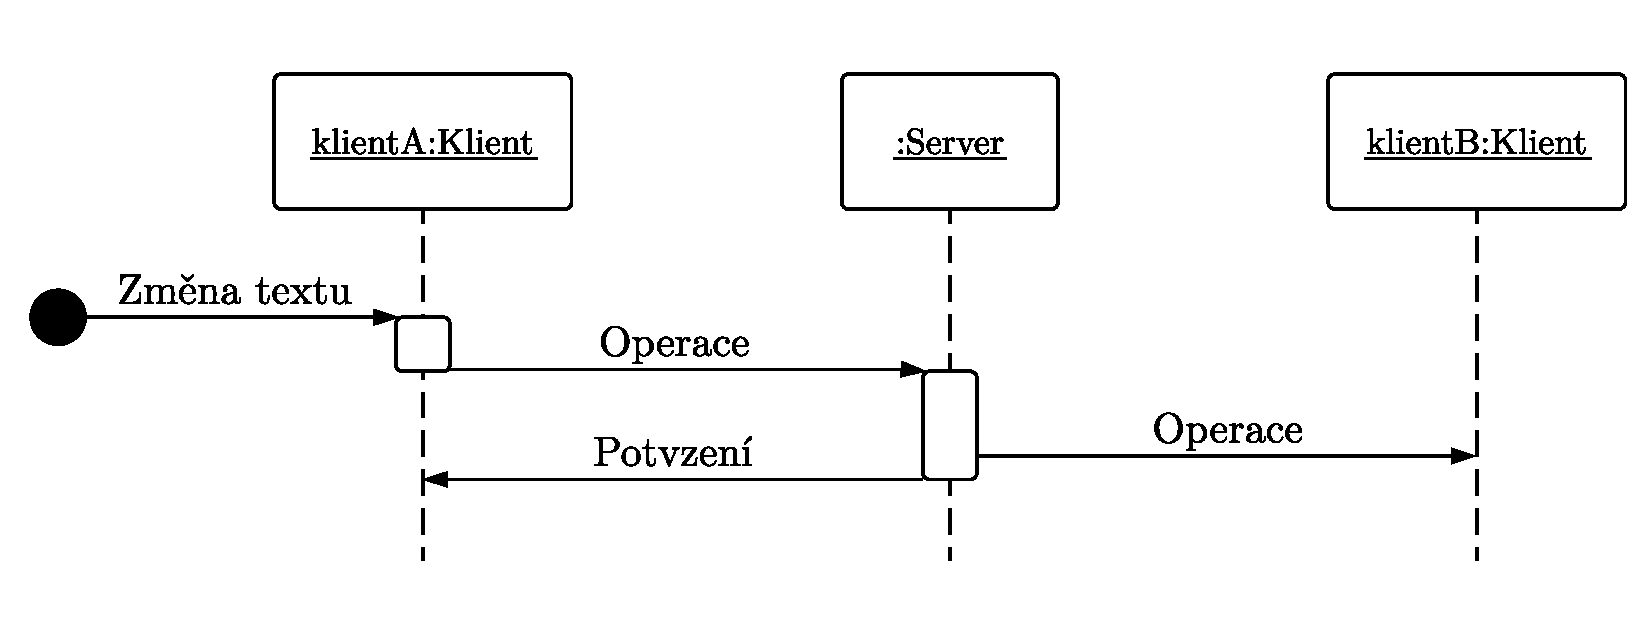
\includegraphics[width=\textwidth]{partials/navrh/ukazkaKomunikaceVeSkutečnémČase.pdf}
    \caption{Sekvenční diagram ukázka komunikace po změně dokumentu}\label{fig:ukazkaKomunikaceVeSkutečnémČase}
\end{figure}

\subsubsection{Potvrzení} % ack()

Zprávu Potvrzení odešle server klientovi jako odpověď na nově zaslanou zprávu Operace, po té co ji zpracuje.
Klient do doby přijetí zprávy Potvrzení nesmí odeslat na server další zprávu Operace (viz sekce~\ref{subsec:klientskáČást}).

\subsubsection{Vybrání} % selection(selection)

Zpráva Vybrání slouží pro propagaci změny kurzoru (či vybrání části textu) mezi klienty.
Server tuto zprávu nijak nezpracovává a pouze ji propaguje ostatním klientům.

Tato zpráva je použita pouze v případě, že se změnila pozice kurzoru bez změny textu (změna pozice kurzoru při změně textu je již obsažena ve zprávě Operace).

\subsubsection{Nastavení} % settings(settings)

Zpráva Nastavení slouží pro synchronizaci změn nastavení mezi aktuálně připojenými klienty upravující stejný dokument.
Klient zprávu odešle spolu se změněným nastavením dokumentu, server nastavení pro daný dokument uloží a následovně jej odešle ostatním připojeným klientům.

\subsubsection{Zpráva} % chat_message(message, callback)

Tento druh zprávy slouží pro propagaci nových zpráv komunikačního vlákna dokumentu.
Klient odešle zprávu s textem na server, ten ji uloží a odešle ostatním připojeným klientům.

Tento způsob propagace zpráv komunikačního vlákna je kombinován s \gls{REST} koncovými body (viz sekce~\ref{sec:restKomunikace}), které umožňují klientům získat například historii komunikačního vlákna.

\subsubsection{Chyba} % disconnect_error(status)

Zpráva Chyba předchází násilnému odpojení klienta od serveru (a tedy od dokumentu).
Její příčinou může být například nedostatečné oprávnění uživatele, či nenalezení příslušného dokumentu.

Součástí zprávy Chyba je stavový kód chyby, který může nabývat hodnot 404 nebo 403.
Hodnota 404 značí, že nebyl nalezen požadovaný dokument nebo k němu neměl uživatel oprávnění.
Hodnota 403 značí, že uživatel provedl operaci, ke které neměl dostatečné oprávnění.
